\section{Model/Implementation Details}\label{sec:3-model}

\subsection{Programming Language}

This is programmed in C++, as the C family of languages are what I am familiar with, and speed is the name of the game here, due to the immense number of calls to complex mathematical routines.

\subsection{Dependencies}

There are two main dependencies that are used, and those are \href{http://gnuplot.info/}{Gnuplot} and \href{https://www.lhapdf.org/}{LHAPDF}. Gnuplot is a simple command-line tool used for plotting data, and it will allow me to visualize results very easily and nicely, and have them be comparable to results from other frameworks. \textsc{LHAPDF} is a package used to interface with PDFs. The reason why this must be done with a library like this is because PDFs are not calculable: they must be fitted from experimental data. Also, there is one caveat with this library, and it is that it cannot be built/used on Windows, unless you use Windows Subsystem for Linux.


\subsection{Structure and Diagrams}

\begin{figure}[ht]
  \centering
  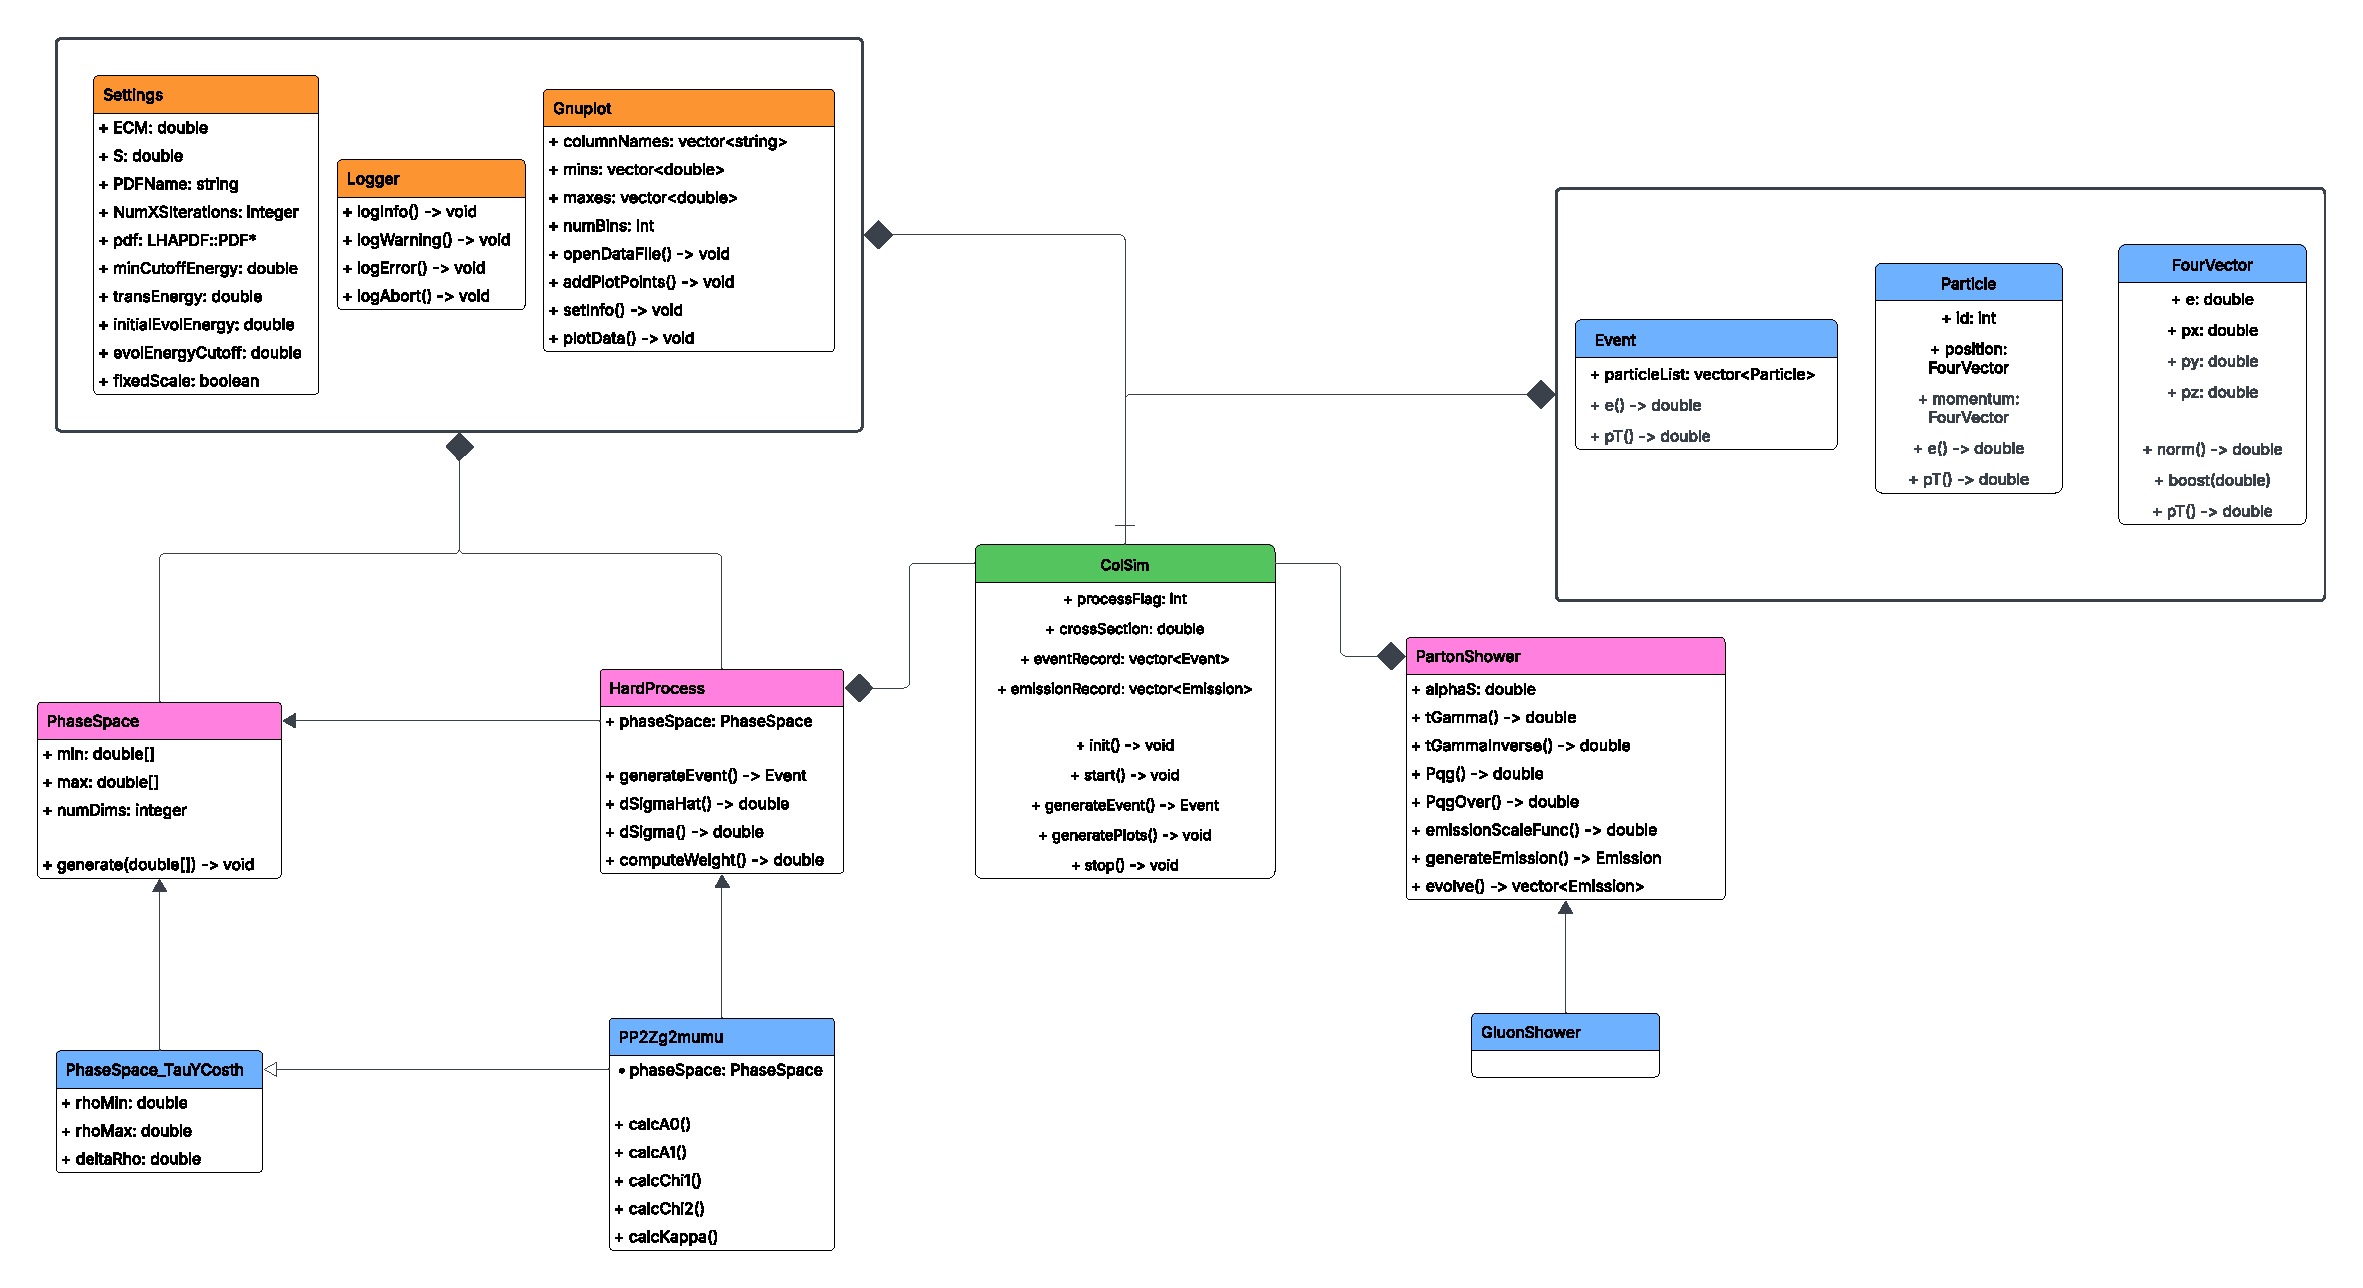
\includegraphics[width=0.9\linewidth]{./res/gfx/ColSim_Updated2.pdf}
  \caption{Basic UML diagram describing the interaction/relationships between the different classes.}
  \label{fig:3-model-uml}
\end{figure}


Given in Fig.~\ref{fig:3-model-uml} is a UML diagram representing the main interacting parts of the program. The blocks listed in orange are singleton classes containing functionality that should be available throughout the program via a single interface. The \mintinline{cpp}{Logger} is a class designed at nicely formatting output to a log file and/or standard output/error. In particular, output is given a prefix stating the severity/priority of the message, since some messages are simply messages whereas some are warnings or errors, as well as a time it was outputted, and if your terminal supports it, colors. Further, if an error is serious enough, \mintinline{cpp}{logAbort()} will stop program execution.

The \mintinline{cpp}{Settings} class contains things related to reading in data from the configuration file, parsing it, and making it available throughout the program. It also contains other generic, configurable parameters.

The blue blocks are separate classes with no dependencies themselves as they are simple organization of numbers. In particular, this is where data related to particles such as ID, momentum, and so on are stored as well as groups of particles, weight information, and so on. These are referenced throughout the program, most notably in the \mintinline{cpp}{Event}/\mintinline{cpp}{Emission} classes, which are organized lists of particles.

The pink blocks are base classes representing generic behavior for that type of object. The \mintinline{cpp}{PartonShower} class defines common behavior such as the implementation of the Sudakov form factor which should be common for all types of parton showering, should more be implemented in the future. Similarly, the \mintinline{cpp}{HardProcess} and \mintinline{cpp}{PhaseSpace} classes contain shared information for all hard process and all of their phase spaces.

Lastly, the single green block, representing the \mintinline{cpp}{ColSimMain} class, is the main entry point for the user, containing simple methods to initialize the program, generate events, and view output.


\subsubsection{Brief Implementation Demonstration}

Here I briefly show a specific instance of some of the implementations described above and shown in the UML diagram in Figure~\ref{fig:3-model-uml}, I show here the behavior for the calculation of the hard scattering cross section. By defining the base \mintinline{cpp}{HardProcess} class, additional processes are able to simply inherit from this class, making it very simple to add new processes (unfortunately the process itself is almost certainly going to be a challenge to implement) so long as they return the required information, namely the cross section, the error, the maximum value of the cross section (to be used for the hit-or-miss method), and the phase space points corresponding to the maximum cross section.

It is done this way so that, in \mintinline{cpp}{ColSimMain}'s \mintinline{cpp}{start()} method, all that we need to include is the code given in Listing~\ref{listing:3-model-start}.

\begin{listing}[ht]
\begin{minted}{cpp}
// set phase space ranges according to input parameters
hardProcess->getPhaseSpace().setRanges();

// calculate the cross section
LOGGER.logMessage("Calculating cross section via Monte Carlo integration...");
HardProcessResult res = hardProcess->calculate();
LOGGER.logMessage("Finished!");
LOGGER.logMessage("Result is: %.9lf +- %.9lf pb (picobarns)",
				  res.result, res.error);

// store values, errors, and phase space points
// corresponding to the maximum weight achived
crossSection = res.result;
crossSectionError = res.error;
maxWeight = res.maxWeight;
maxPSPoints = res.maxPoints;

LOGGER.logMessage("Maximum weight achieved: %.9lf", maxWeight);
\end{minted}
\caption{The main code run within \mintinline{cpp}{ColSimMain}'s \mintinline{cpp}{start()} function to calculate the cross section.}
\label{listing:3-model-start}
\end{listing}

The code for generating parton showering events is of course different, but still simple and allows for the implementation of additional events, so long as they return an array of \mintinline{cpp}{Emissions} encoding the quark's energies at each emission and the kinematics of the emitted gluons (which, in general, could be photons as well).

It is worth noting that the Logger functionality is also present here; the capital \mintinline{cpp}{LOGGER} is a macro defined like so:

\begin{minted}{cpp}
#define LOGGER Logger::getInstance()
\end{minted}

As a singleton, then, the logger functionality is now available, as a single instance, to the entire program, avoiding duplications or truly global variables. The Settings functionality is encoded in a very similar way.

We are also able to see similar behavior for the phase space: different cross sections can be encoded in terms of different phase space variables; sometimes variable transformations may make calculations easier. Either way, the phase space functionality is implemented in a nearly identical way: the main \mintinline{cpp}{PhaseSpace} class contains the names, minimums, maximums, and ranges for all of the that particular phase space's variables. It interfaces with the \mintinline{cpp}{Settings} singleton class to update ranges whenever values are input parameters are changed, and spits out randomly generated values (scaled appropriately) to be used in the calculation of the cross section.


\subsection{Execution Instructions}

\textsc{ColSim} was made as a library, so it can be interfaced with via a C++ program, as opposed to a single executable. An example main file is given in Listing~\ref{listing:colsim-main}.

\begin{listing}[!ht]
\begin{minted}{cpp}
#include "ColSim/ColSim.hpp"
using namespace ColSim;
using namespace std;

#include <iostream>

int main() {
  // create the main object
  ColSimMain colsim;

  colsim.init(ColSimMain::HARD_PROCESS);

  // start/initialize generation
  colsim.start();

  // generate events
  colsim.generateEvents(100000);
	
  // generate the plots
  colsim.generatePlots();

  // stop/deinitialize generation
  colsim.stop();
    
  return 0;
}
\end{minted}
\caption{An example main program interfacing with ColSim and generating 100000 hard scattering events.}
\label{listing:colsim-main}
\end{listing}

The user first creates a \mintinline{cpp}{ColSimMain} object and initializes it for hard scattering. In between \mintinline{cpp}{start()} and \mintinline{cpp}{stop()} commands, we generate 100000 events and also generate plots. To generate events for parton showering, one can pass in the flag \mintinline{cpp}{ColSimMain::PARTON_SHOWER}. Both types of outputs are described in a subsequent section.

\subsubsection{LHAPDF}\label{sec:3-model-lhapdf}

Before continuing, \href{https://www.lhapdf.org/}{LHAPDF} must be installed on your system. As described previously, it is a library to allow for interfacing with PDFs, and is required for \textsc{ColSim}. Installation instructions are on their website, and are relatively straightforward. To reiterate: \textbf{this library can only be build on Unix-like systems; it cannot be used on Windows without WSL.} Once the library is installed and your system paths are set up appropriately, PDFs can be installed by using the \texttt{lhapdf} command line tool. For instance, to install the CT18NNLO PDF set (the default for \textsc{ColSim}), one can run

\begin{minted}{bash}
lhapdf install CT18NNLO
\end{minted}

in their shell.

\subsubsection{Gnuplot}

Gnuplot is far easier to install, as it is included in most package managers. For instance, Debian-based systems need only type

\begin{minted}{bash}
sudo apt-get install gnuplot
\end{minted}

to have all required functionality. A quick check would be to ensure the \texttt{gnuplot} command line tool works by running

\begin{minted}{bash}
gnuplot --help
\end{minted}


\subsubsection{Compiling}

Clone the \href{https://github.com/champso1/ColSim}{repository} somewhere, and cd into it. You can then follow standard CMake building:

\begin{minted}{bash}
  mkdir build
  cd build
  cmake .. -DLHAPDF_ROOT_DIR=<path-to-LHAPDF>
  cmake --build .
  cmake --install .
\end{minted}

The default path for binary installation is \texttt{/path/to/ColSim/install}, which lies within the project directory. This way, building and running the examples are very simple. Again, ensure that CMake can find LHAPDF's files. If they were not installed to standard system paths, you can set the \texttt{LHAPDF\_ROOT\_DIR} variable in your shell's environment or by passing its installation prefix to CMake, like above.

\subsubsection{Running}

Once \textsc{ColSim} is built and installed to your location of choosing, it can be used like any other library. In the \texttt{examples} folder in the repository is an example called ``basic'' which simply generates $\num{100000}$ hard scattering events and plots the kinematics (these will be described in Section~\ref{sec:4-results}). It it also built via the standard CMake building procedure, but of course without the installation step. An executable titled \texttt{basic} will be spit out in the build folder.

\subsubsection{Configuration File}

In the \texttt{res} directory at the top level of the project is a file titled \texttt{config.in}, which is a configuration file containing the default values for all of the input parameters for the model. Since these are all defaults, \textsc{ColSim} does not require a configuration file, but it can be copied to the same directory as the executable for the given example, and, if passing the name of the file to \mintinline{cpp}{ColSimMain}'s constructor, will read values from the file. One can also use the \mintinline{cpp}{readString()} method in the \mintinline{cpp}{Settings} class within the code to change input parameters if one does not want to use a configuration file. The entire file is given in Listing~\ref{listing:colsim-config-file} in Appendix~\ref{sec:colsim-config-file}, as it is a bit large to display here. Also in the listing are descriptions for each variable, but for ease of viewing, we also present them here in the next (sub)section with a bit more information than what is included in the default configuration file.



\subsubsection{Configurable Parameters}

There is one generic parameter used for both hard scattering and parton showering:

\begin{itemize}
\item \textbf{PDFName}: The name of the parton distribution function (PDF) set to use. Different PDFs report information with different accuracy, including different effects, and so on. For the purposes of this program, most any popular PDF set is valid; the default is set to the CTEQ collaboration's NNLO set: \texttt{CT18NNLO}. If one wants to use other PDF sets, navigate \href{https://lhapdf.hepforge.org/pdfsets.html}{here} to see the available list and invoke the command line tool like so:
\begin{minted}{bash}
lhapdf install <PDF-set-of-choice>
\end{minted}
\end{itemize}

The hard scattering process has four configurable parameters:

\begin{itemize}
\item \textbf{NumXSIterations}: The number of Monte Carlo iterations to do in the computation of the cross section. This parameter of course carries no physical significance, but higher numbers reduce error and vice versa. The default is one million, but on my machine this already runs in under a second, so higher iterations are very feasible to give very accurate results.
\item \textbf{ECM} ($E_{\mathrm{CM}}$): The center-of-mass energy for the proton-proton collision, or in other words, each proton carries $E_{\mathrm{CM}}/2$. This is set to $\qty{14.0}{\TeV}$ as this is the current $E_{\mathrm{CM}}$ that the LHC in CERN is running collisions at. Higher $E_{\mathrm{CM}}$s shift most energy/momentum-based distributions to the right.
\item \textbf{MinCutoffEnergy}: The energy cutoff imposed during the cros section calculation. There is an absolute cutoff before the entire theory on which these calculations are based breakdown; this is around $\mathcal{O}(\qty{~1.0}{\GeV})$, as described in Section~\ref{sec:2-theory-cutoff}. Due to the larger energy scale of the main interaction, we can afford to set this cutoff a bit higher to increase computational efficiency, but this can in principle be set as low or high as one desires, with accuracy impacts.
\item \textbf{TransformationEnergy}: An intermediate calculational parameter that is usually kept around $\qty{~60}{\GeV}$, or roughly around the minimum cutoff energy. As we will see in Section~\ref{sec:5-sensitivity-scenario}, values too much lower/higher cause odd behavior and divergences. This value is introduced as a transformation parameter as described in Section~\ref{sec:2-hit-or-miss} in order to use the hit-or-miss method more easily. Hence, it has no physical meaning, but is left configurable.
\end{itemize}


The parton showering parameters are as follows:

\begin{itemize}
\item \textbf{InitialEvolEnergy}: The initial energy that the quark has before undergoing its evolution. This is usually set to the be roughly the energy scale of a generic subprocess of the main proton-proton collision which is roughly $\mathcal{O}(\qty{~1}{\TeV})$; this is the default value.
\item \textbf{FixedScale}: This is a Yes/No parameter. The value of the coupling term $\alpha_s$ for the interaction between the quarks and the gluons in principle changes with the energy scale, but not enough in this regime to substantially impact the physics. Of course, letting it vary with the quark's energy scale leads to slightly higher accuracy, but again, the impact is not significant enough to motivate me to keep it one way or the other.
\item \textbf{EvolutionEnergyCutoff}: As described earlier, this cutoff is due to the fact that at lower energies than this our theory breaks down. Here, since we are directly evolving the quark to these low energies we want to have this cutoff be at the absolute minimum to capture as many emissions as possible. The code will actually error out if the user tries to set this to a value lower than $\qty{1}{\GeV}$ and warns for a value $\qty{>10}{\GeV}$.
\end{itemize}








%%% Local Variables:
%%% mode: LaTeX
%%% TeX-master: "../../FinalMilestone"
%%% End:
